
\chapter{Experimentación y resultados}
\label{chap:experimentation}
Una vez que hemos desarrollado un software específico para aproximar la órbita de un objeto mediante el método de Laplace, comprobemos su correcto funcionamiento, así como cómo de buenas son los las aproximaciones obtenidas con el método Laplaciano (objetivo 8).\\

Dado que no disponemos de instrumental óptimo para realizar las observaciones por nuestra cuenta, utilizaremos (una vez más) la efemérides online del JPL \cite{jpl}, con la que podemos obtener la ascensión recta y declinación observada desde la Tierra de cualquier objeto en cualquier momento. De esta manera, comencemos a ver diferentes resultados prácticos y comentemos la eficacia del método de Laplace que hemos estudiado.\\

\section{Cuando el cuerpo es cercano: Ceres.}
\label{sec:exp_ceres}
Tal y como hemos comentado en \ref{sec:history}, en 1801 Giuseppe Piazzi descubría el planeta enano Ceres, y meses más tarde Gauss usaba su recientemente desarrollado método para obtener la órbita del objeto con las observaciones que Piazzi había anotado. Gracias a ello, pudieron recuperar la pista de este planeta enano.\\

En ese momento quedó demostrado que el método de Gauss hacía buenas estimaciones para cuerpos a una distancia aproximada a la de Ceres. ¿Hubiera conseguido Laplace unos resultados exitosos? Veámoslo.\\

Vamos a tomar la ascensión recta y declinación de Ceres para ciertos momentos entre los días 28 y 30 de julio de 2020. Los introducimos en el programa desarrollado junto a su nombre, quedando de la siguiente manera:
\begin{figure}[H]
\centering
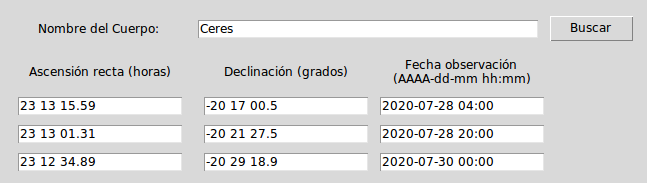
\includegraphics[scale=0.5]{images/ceres_exp.png}
\caption{Datos de Ceres introducidos en el programa.}
\label{fig:ceres_exp}
\end{figure}

Cuando pulsemos el botón ``Buscar'' encontrará en la efemérides los valores del cuerpo requerido de manera satisfactoria.
\begin{lstlisting}[style=Console]
Órbita de Ceres obtenida.
Ahora puedes dibujar el objeto junto al resto.

Nombre = 'Ceres'
a = 2.7672121143653663 UA
e = 0.07772816968324102
i = 10.588147218912999 grados
(*$\Omega$*) = 80.28170111757919 grados
(*$\omega$*) = 73.71539237319364 grados
Período = 1681.3979070284568 días
\end{lstlisting}

A continuación, veamos qué tal funciona el método de Laplace. Con dichos valores, obtenemos los siguientes posibles valores para $\phi$:
\[
\left\{
\begin{array}{l}
\phi_1=11.9311189º\\
\phi_2=37.60583084º\\
\phi_3=134.04867322º
\end{array}
\right.
\]

Dado que $\psi=142.39416916267487º$, cuando calculemos $\pi-\psi$ veremos que es igual a $\phi_2$, por lo que la solución será única y se corresponderá con $\phi_1$.\\

En vez de mostrar el resultado de aplicar el método laplaciano y calcular los elementos orbitales (será más visual compararlo en una gráfica), veamos directamente el error con su valor real utilizando el botón ``Error'':
\begin{lstlisting}[style=Console]
Posición real: [ 2.53436621 -1.48439324 -0.51379219]
Posición calculada: [ 2.54870673 -1.48940124 -0.51764288]
Error = [-0.01434052  0.005008    0.00385069]
|Error| = 0.01567030503509054

Velocidad real: [ 0.00478149  0.00826443 -0.0006202 ]
Velocidad calculada: [ 0.00496131  0.00816816 -0.00068937]
Error = [-1.79816103e-04  9.62781299e-05  6.91715556e-05]
|Error| = 0.0002153787671514888

Distancia real: 2.9816803651312407
Distancia aproximada: 2.9970278967029773
\end{lstlisting}

Podemos observar que la aproximación en $t=$2020-07-28 20:00 es muy buena a pesar de que se haya realizado con tan solo tres observaciones del cuerpo desde la Tierra. Aún así, hay que tener en cuenta que un error en la distancia de $0.01$ UA se corresponde con $1495978.707$ kilómetros.\\

Para terminar, utilicemos las coordenadas astronómicas que hemos aproximado de Ceres para dibujar la órbita asociada a estas coordenadas. Además, añadiremos la órbita real para comprobar cómo de buena es la aproximación, y la órbita de la Tierra para hacernos una pequeña idea de la distancia del cuerpo que hemos utilizado.

\begin{figure}[H]
\centering
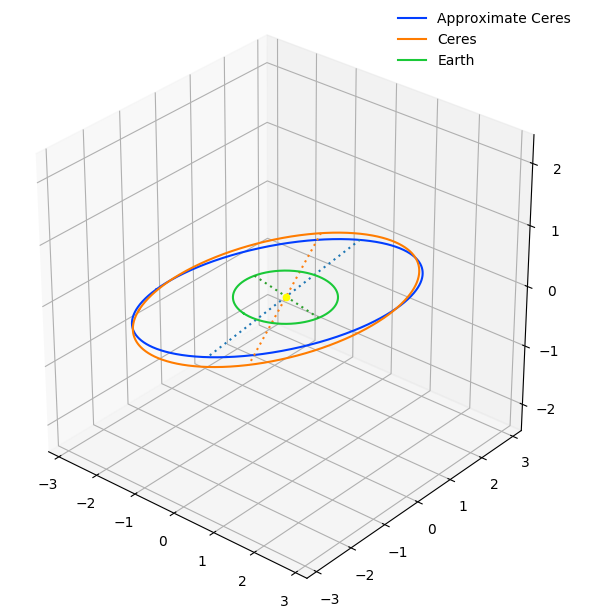
\includegraphics[scale=0.35]{images/plot_ceres.png}
\caption{Órbita real y aproximada de Ceres junto a la Tierra.}
\label{fig:plot_ceres}
\end{figure}

Es fácilmente observable que los elementos orbitales obtenidos a través de la aproximación son muy similares a los reales, y con dicha órbita aproximada podríamos encontrar el planeta enano Ceres en la bóveda celeste. Por tanto, el método de Laplace hubiera sido tan válido como el de Gauss para que en 1801 se hubiese recuperado el cuerpo en el cielo nocturno.\\

\section{El error aumenta con la distancia: Hilda y Plutón.}
\label{sec:exp_hilda_pluton}
Ya hemos visto que con un cuerpo relativamente cercano funciona bien el método de Laplace. Alejémonos un poco más.\\

Empecemos tomando el asteroide Hilda (A875 VC en la efemérides), un objeto que da nombre a un grupo de asteroides situado a unas cuatro unidades astronómicas, entre la órbita de Júpiter y el cinturón de asteroides. Tomamos su ascensión recta y declinación de la efemérides en un intervalo de unos dos días, las introducimos en el programa y aplicamos el método de Laplace.\\

\begin{figure}[H]
\centering
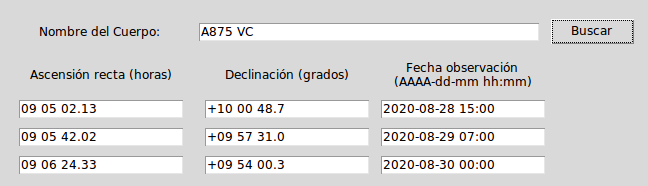
\includegraphics[scale=0.5]{images/hilda_exp.png}
\caption{Datos de Hilda (A875 VC) introducidos en el programa.}
\label{fig:hilda_exp}
\end{figure}

Antes de dar un resultado para la posición y velocidad del cuerpo, el programa para, ya que ha encontrado una solución doble, y nos pregunta sobre cuál de los dos valores posibles queremos tomar como solución del problema físico.\\
\[
\left\{
\begin{array}{l}
\phi_1=4.35491299º\\
\phi_2=18.19187998º\\
\phi_3=158.82202981º=\pi-\psi
\end{array}
\right.
\]

Si escogiésemos $\phi_2$ estaríamos tomando un ángulo mayor al que se encontró como solución en el caso de Ceres, lo cuál no tendría sentido, pues a mayor distancia del cuerpo, menor ángulo forma con la Tierra y el Sol; por tanto, elegiremos como solución $\phi_1$. Nótese que este razonamiento no se podría haber hecho en un caso real de determinación de órbitas, pues a priori no sabemos si el objeto está mas cerca o más lejos con una simple observación.\\

Veamos el resultado que se obtiene tras discernir entre cuál de las dos soluciones es la buena:
\begin{lstlisting}[style=Console]
Aproximación en t = 2020-08-29 07:00:00.000
Posición calculada: [-3.16680643  3.55611002 -0.63839816]
Velocidad calculada: [-6.72694445e-03 -7.39134996e-03 -6.61539321e-05]

Elementos orbitales obtenidos:
Nombre = 'Approximate A875 VC'
a = 12.704405560669025 UA
e = 0.6270295383846635
i = 7.72591356505979 grados
(*$\Omega$*) = 129.50904027965768 grados
(*$\omega$*) = 276.6199742996565 grados
Período = 16540.108377222892 días
\end{lstlisting}

\begin{lstlisting}[style=Console]
Posición real: [-2.83281544  3.23203176 -0.58633104]
Posición calculada: [-3.16680643  3.55611002 -0.63839816]
Error = [ 0.33399099 -0.32407826  0.05206712]
|Error| = 0.46828163075398077

Velocidad real: [-5.32298460e-03 -5.80807100e-03 -1.18918535e-05]
Velocidad calculada: [-6.72694445e-03 -7.39134996e-03 -6.61539321e-05]
Error = [1.40395985e-03 1.58327896e-03 5.42620785e-05]
|Error| = 0.002116794723497365

Distancia real: 4.337586507139335
Distancia aproximada: 4.804386918636096
\end{lstlisting}

Aunque el error en la aproximación de la posición y la velocidad no es excesivamente grande, parece que la cosa no ha ido demasiado bien a la hora de pasar a coordenadas astronómicas, pues habíamos comentado previamente que la distancia del asteroide al Sol era aproximadamente 4 UA, mientras que hemos obtenido una distancia de 12 UA. Veamos una imagen de la órbita calculada junto a la real y las órbitas de la Tierra y Júpiter.

\begin{figure}[H]
\centering
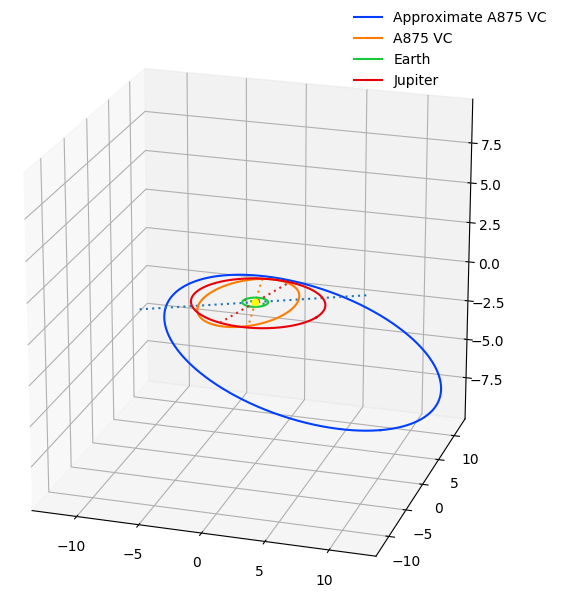
\includegraphics[scale=0.35]{images/hilda_plot.png}
\caption{Órbita real y aproximada de Hilda (A875 VC) junto a la Tierra y Júpiter.}
\label{fig:hilda_plot}
\end{figure}

La aproximación ha sido bastante mala, por lo que no sería mala idea probar con otras observaciones, teniendo en cuenta que podríamos tomarlas más o menos espaciadas que en el caso que hemos estudiado.\\

Comprobemos rápidamente si alejándonos más todavía del Sol sigue aumentando el error de aproximación. Vayámonos muy lejos, concretamente a Plutón. Tomemos sus coordenadas ecuatoriales en tres momentos diferentes y veamos qué tal se porta el método de Laplace.\\

El método se aplica y obtiene una solución de $\phi$ única; en vez de mostrar todo el error, veamos solamente qué tal ha aproximado la distancia al planeta en $t=$2020-09-14 19:00.

\begin{lstlisting}[style=Console]
Posición real: [ 13.74165616 -31.22436196  -0.6327821 ]
Posición calculada: [  7.74035668 -16.5876921   -0.33519062]
Error = [  6.00129948 -14.63666986  -0.29759148]
|Error| = 15.822018227154214
\end{lstlisting}

Con esto podemos ir empezando a sospechar que, mientras mantengamos el intervalo de toma de observaciones, cuanto mayor sea la distancia al cuerpo observado, mayor será el error que acarrea la aproximación de su posición y velocidad. Es más, el error en esta aproximación hará que al calcular los elementos orbitales obtengamos un semieje mayor negativo, algo que no es posible, y esta aproximación debería ser descartada como solución del problema físico.

\begin{lstlisting}[style=Console]
Aproximación en [...]

Elementos orbitales obtenidos:
Nombre = 'Approximate 999'
a = -0.0019409803348728837 UA
e = 581.0174156903244
[...]

Semieje mayor negativo, no se puede dibujar la órbita.
\end{lstlisting}

\subsection{Intentando solucionar el problema de la distancia.}
No conformes con el resultado que hemos obtenido en la aproximación de objetos más lejanos, veamos si podemos arreglar el error tan grande que se produce. Comprobando los valores de las derivadas $(\lambda,\mu,\nu)$ durante el proceso de aproximación, vemos que los valores que toman son muy pequeños. Por tanto, empezamos a suponer que el error reside aquí.\\

Cuando observamos un cuerpo muy lejano a la Tierra, podemos ver que su posición varía poquísimo entre un día y otro (aparentemente). Para que la posición entre dos observaciones cambien más, debemos de escoger un intervalo de tiempo mucho más grande entre cada toma de datos. Y eso es lo que vamos a hacer ahora.\\

Tomemos de nuevo el planeta enano Plutón e introduzcamos en nuestro software los valores de ascensión recta y declinación con una diferencia entre cada medida de un mes (seis de marzo, seis de abril y seis de mayo). Al aplicar el método de Laplace, obtenemos dos soluciones posibles, $\phi_1=1.62991238º$ y $\phi_2=80.67644758$. Si la solución del problema físico fuera $\phi_2$, al ser tan grande el ángulo formado el objeto observado debería de estar muy cerca, pero sabemos que ese no es el caso; por tanto, deducimos que la solución válida es $\phi_1$. La seleccionamos y pasamos a directamente a comprobar el error de la aproximación.
\begin{lstlisting}[style=Console]
Posición real: [ 13.26236291 -31.31779618  -0.48455854]
Posición calculada: [ 13.59730661 -32.05011445  -0.4966634 ]
Error = [-0.3349437   0.73231826  0.01210486]
|Error| = 0.8053718719482896

Velocidad real: [ 0.0029688   0.00056318 -0.00090387]
Velocidad calculada: [ 0.00291106  0.00065941 -0.00093223]
Error = [ 5.77378776e-05 -9.62253998e-05  2.83582814e-05]
|Error| = 0.0001157461974060685

Distancia real: 34.013665264543306
Distancia aproximada: 34.818719933147946
\end{lstlisting}

En esta ocasión, los resultados son mucho más prometedores que haciendo las observaciones más cercanas, con una velocidad muy cercana y una posición con ``solo'' una unidad astronómica de error, que para la distancia a la que estamos trabajando está bastante bien. Veamos si hemos tenido la misma suerte con los elementos orbitales.

\begin{figure}[H]
\centering
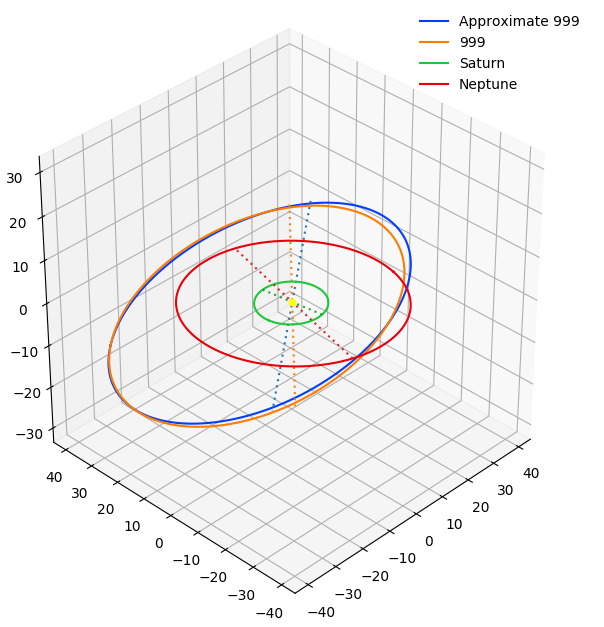
\includegraphics[scale=0.35]{images/plot_pluto_ok.png}
\caption{Órbita real y aproximada de Plutón (999) junto a la Saturno y Urano.}
\label{fig:plot_pluto_ok}
\end{figure}

La órbita real y aproximada son muy similares, por lo que podemos concluir que la decisión de tomar observaciones más espaciadas en el tiempo es una buena elección cuando el cuerpo se encuentra muy alejado de la Tierra. Aún así, en un caso real no sabemos si el cuerpo está más o menos cerca del observador, por lo que la elección del intervalo de tiempo entre cada toma debe de ser estudiada antes.\\



\section{Órbitas muy excéntricas: C/2020 F3 (Neowise).}
\label{sec:neowise}
Cuanto mayor sea la excentricidad de un cuerpo espacial, más alejado estarán sus focos, pero más se acercará a ellos en algún momento de su órbita. Este es el caso del objeto C/2020 F3 (Neowise), un cometa del que se oyó mucho hablar durante el pasado mes de julio debido a que, en su trayectoria alrededor del Sol, se acercaba al punto más cercano a la Tierra, de manera que se podía observar a simple vista, y no volvería a ser así hasta dentro de 6765 años.\\

Hemos visto que con objetos muy lejanos e intervalos muy pequeños para las observaciones, la aproximación que nos da el método de Laplace es muy mala. Pero, ¿y si las medidas se toman cuándo el objeto esté muy cercano a la Tierra, de manera que las observaciones sean incluso mejores que las de Ceres?\\

Escogemos los valores de las observaciones del cometa entre el día 14 y el día 15 de julio, en los que su posición en la órbita se encontraba muy cerca de la Tierra.
\begin{figure}[H]
\centering
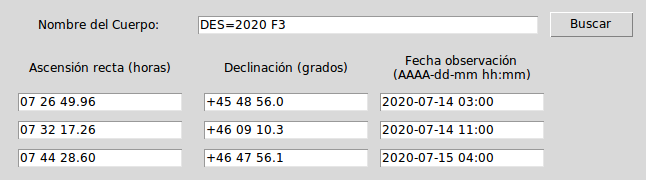
\includegraphics[scale=0.5]{images/neowise_exp.png}
\caption{Datos de C/2020 F3 (Neowise) introducidos en el programa.}
\label{fig:neowise_exp}
\end{figure}

Al aplicar el método de Laplace, volvemos a obtener una solución doble, $\phi_1=90.35678364º$ y $\phi_2=107.33111728º$. En este caso no podemos decidir fácilmente entre cuál de las dos es la válida por lo que elegimos, por ejemplo, $\phi_2$ (y tendremos suerte con la elección). Tras la ejecución, comprobamos el error con la posición y velocidad real en el instante que hemos aproximado.
\begin{lstlisting}[style=Console]
Posición real: [ 0.16652972 -0.24402154  0.32665628]
Posición calculada: [ 0.16854806 -0.25029356  0.32362519]
Error = [-0.00201834  0.00627202  0.00303109]
|Error| = 0.0072525445535108184

Velocidad real: [-0.01084886 -0.03392851  0.00860642]
Velocidad calculada: [-0.0106734  -0.03331783  0.00864502]
Error = [-1.75460689e-04 -6.10680287e-04 -3.85976705e-05]
|Error| = 0.0006365584389714605

Distancia real: 0.44043499684292076
Distancia aproximada: 0.4424800312802405
\end{lstlisting}

Como vemos, los errores al calcular los vectores de posición y velocidad son muy pequeños, hecho que era de esperar al estar tan cerca el objeto que se ha observado. ¿Tendremos la misma suerte con el cálculo de los elementos orbitales?,\\

Comencemos viendo qué tal ha ido la aproximación para la excentricidad y los ángulos $i$, $\Omega$ y $\omega$, comparando los valores en la siguiente tabla.
\begin{table}[H]
\centering
\resizebox{8cm}{!}{%
\begin{tabular}{cc|c}
         & \textit{Valor real}         & \textit{Valor aproximado}   \\ \hline
$e$      & $0.9992401080381621$ & $0.9623385094824053$ \\ \hline
$i$      & $128.9372837890982$  & $129.87582386324678$ \\ \hline
$\Omega$ & $61.01063124644879$  & $60.32375719162504$  \\ \hline
$\omega$ & $37.28105014282296$  & $34.302810750239566$ \\ \hline
\end{tabular}%
}
\end{table}

Parece que todo ha ido bien, por lo que veamos ahora una imagen comparando las dos órbitas.

\begin{figure}[H]
\centering
\subfloat{
	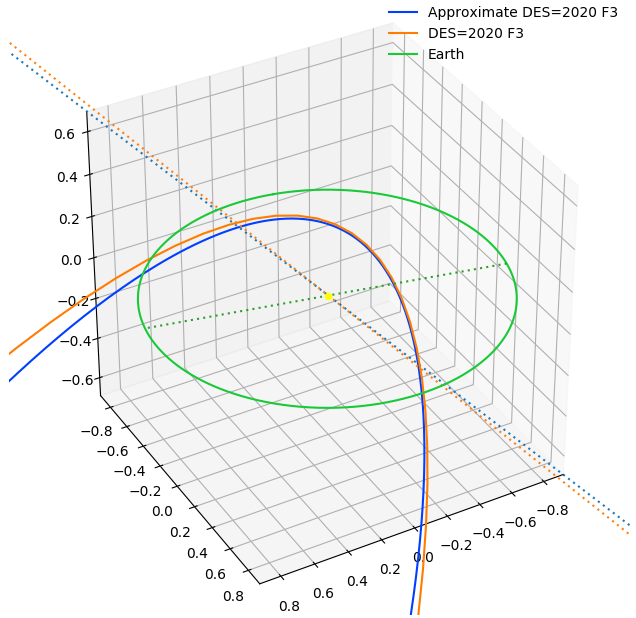
\includegraphics[scale=0.275]{images/neowise_close.png}
	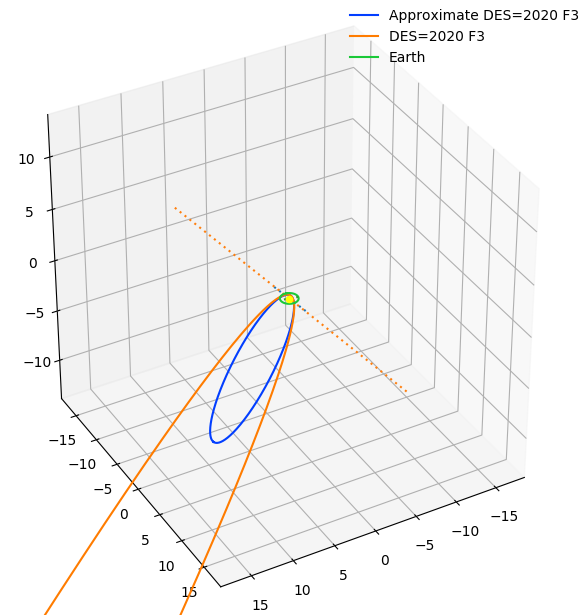
\includegraphics[scale=0.275]{images/neowise_far.png}
}
\caption{Órbita real y aproximada de C/2020 F3 (Neowise) junto a la Tierra vista desde cerca y desde lejos.}
\label{fig:neowise_plot}
\end{figure}

En este caso, observando la órbita de cerca, tenemos una muy buen aproximación, pero conforme nos vamos alejando nos damos cuenta de que ha habido un error muy grande en el semieje mayor: el valor aproximado de $a$ es 7.640204712942875 UA, mientras que el real es de 387.7566248050956 UA, 380 UA de diferencia.\\

Para entender el por qué de este error tan grande tenemos que volver a la sección \ref{sec:elements_determination} y recordar el cálculo de $a$:
\[
h=\frac{|v(t)|^2}{2}-\frac{\mu}{|r(t)|}
\]
\[
a=-\frac{\mu}{2h}
\]

Por tanto, el valor de $a$ depende únicamente del valor de la energía, que se calcula a partir de la norma de la posición y la velocidad. Si tomamos el valor de $a$ como una función en $h$, estaremos ante una función hiperbólica, la cuál divergerá cuando se acerque a 0. Además, para que el valor de $a$ sea muy grande, la energía debe de ser muy cercana a 0. De esta manera, por el hecho de que $a$ diverge en 0, el mínimo error en la energía puede causar un error muy grande en el cálculo del semieje mayor, y esta es la razón del error tan grande obtenido en el semieje mayor del caso de C/2020 F3 (Neowise).


\newpage
\thispagestyle{empty}
